\chapter{Introducción}

Presentar de forma atractiva el trabajo... quizás renombrar el título del trabajo utilizando "all you need", como por ejemplo 

"All you need is sound and music: explorando la interacción creativa con modelos de lenguaje a gran escala en la creación sonora con lenguajes de programación musical"


\begin{figure}[H]
    \caption[Número de publicaciones de \textit{Deep Learning} por año que contienen la expresión <<all you need>> en el título]{Número de publicaciones de \textit{Deep Learning} por año que contienen la expresión <<all you need>> en el título.}
    \centering
    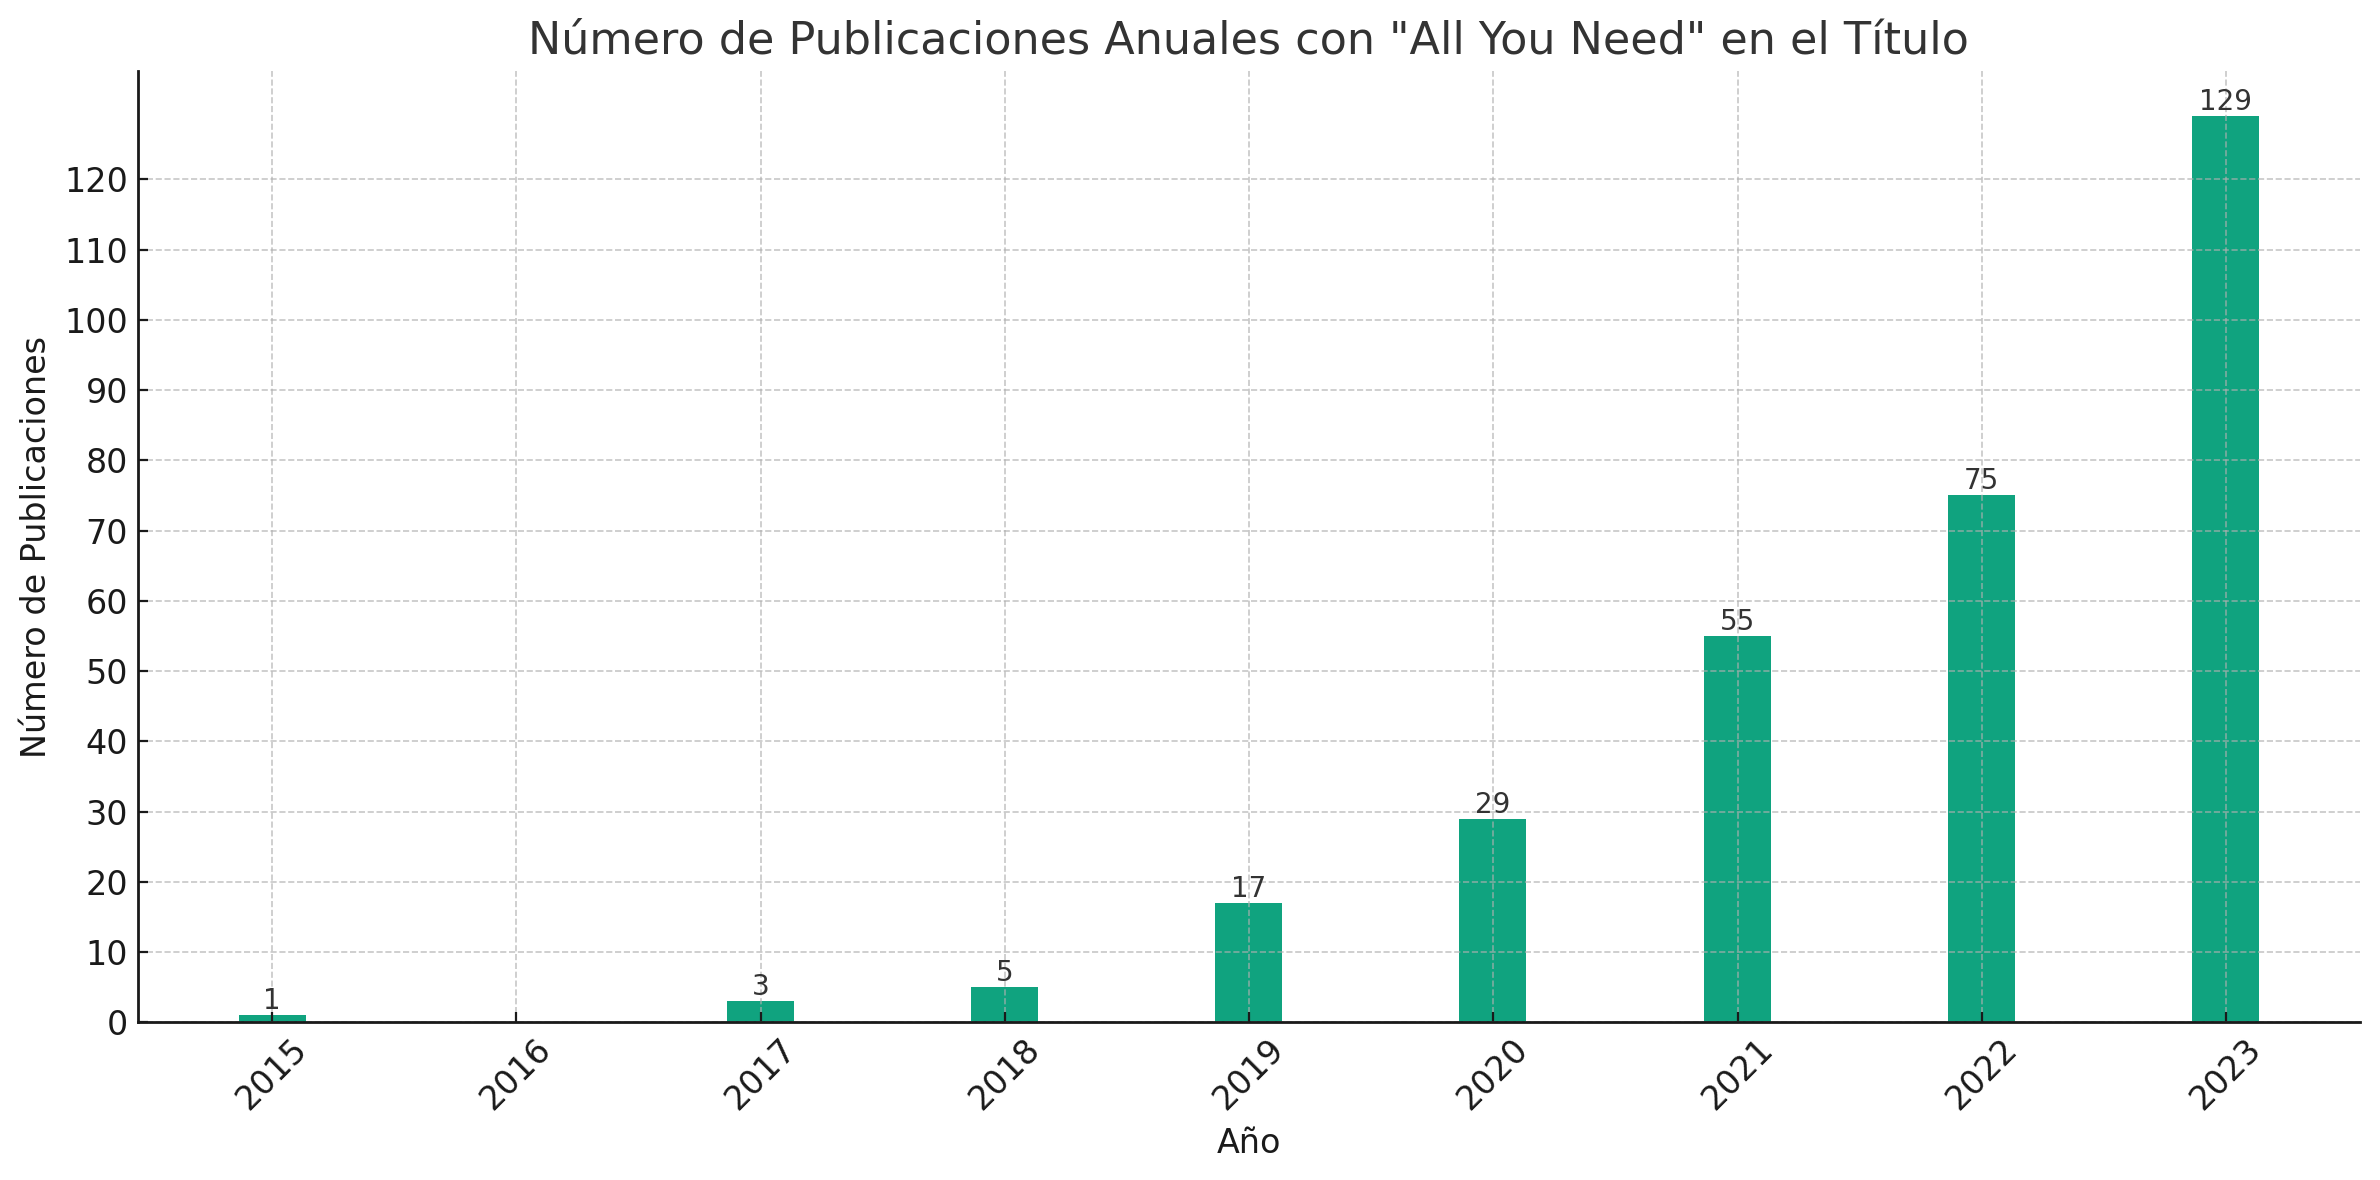
\includegraphics[width=0.9\textwidth]{./figuras/all_you_need_publicacionies_anuales.png}
    \source{Elaboración propia a partir del listado de \url{https://github.com/KentoNishi/awesome-all-you-need-papers}}
    \label{fig:all_you_need_publicaciones}
\end{figure}

\chapter{Justificación}

La evolución de la inteligencia artificial (IA), específicamente dentro del ámbito del \gls{dl}, ha impulsado el desarrollo de Modelos de Lenguaje a Gran Escala (\glsdisp{llm}{LLM}, por sus siglas en inglés, \textit{Large Language Models}) basados en técnicas avanzadas de aprendizaje profundo. Estos modelos, cuyo primer objetivo fue el de modelizar el lenguaje humano, han exhibido capacidades emergentes, como creatividad, razonamiento y habilidades de programación avanzadas. Esto ha impactado en poco tiempo en campos tan variados como la literatura, la programación, el arte visual, la investigación, el marketing, la docencia y, en definitiva, en la mayor parte de las disciplinas que utilizan el lenguaje y el razonamiento.

No sin sorpresa de la comunidad científica, \gls{llm} han demostrado ser particularmente efectivos en la generación de código de programación, lo cual incluye a lenguajes enfocados en la generación musical o sonora, siempre que exista suficiente material en la web con el que entrenar a estos modelos. Sin embargo, la generación de música mediante representaciones simbólicas, como el formato MIDI —el estándar dominante en representación musical digital—, presenta ciertos desafíos para los \gls{llm}. Generar música en dicho formato demanda un conocimiento profundo de teoría musical, armonía, contrapunto y la habilidad de razonar sobre estos elementos, lo cual no se puede dar por supuesto en los \gls{llm} de propósito general, a finales de 2023, no especializados en estas áreas.

No se ignora en este panorama toda la investigación dentro del \gls{dl} relativo al desarrollo de modelos de audio, como \textit{Stability Audio}, \textit{MusicML} de Google o \textit{AWS DeepComposer} de Amazon. Estos modelos generan música (audio) desde texto natural. Los resultados son prometedores especialmente en ámbitos como el marketing, por el eventual abaratamiento de costes en la producción. Sin embargo, estos archivos de audio generados no son editables y escapan al control humano, lo cual limita su uso en la composición musical en la que la figura humana es esencial. Sin embargo, los LLM generan texto a partir de texto. La música representada en código informático es esencialmente texto a pesar de significar un mundo sonoro. El texto generado por los LLM puede ser editado y controlado por el humano. Por tanto, las posibilidades de interacción que se presentan son enormes y son las que se pretenden explorar en este trabajo.

Existen investigaciones centradas en la generación por estos \gls{llm} de algoritmos en lenguajes de programación donde se espera un resultado matemático preciso. Sin embargo, hay un vacío cuando lo que se busca, más allá de la corrección sintáctica, es un resultado artístico alineado con las intenciones del creador de sonido o compositor. No es, ciertamente, lo mismo crear un código de una función que eleve al cuadrado a cualquier input numérico, que crear una función que genere <<el sonido de un bosque en otoño>>. El nivel de comprensión, abstracción, conocimientos previos y contacto con la realidad ha de ser incomparablemente mayor en el segundo caso, incluso cuando su código sea eventualmente más simple que el de una función matemática.

Como se verá, existen decenas de lenguajes de programación enfocados en la creación musical que podrían entrar en consideración en este trabajo. Sin embargo, la investigación se limitará a experimentar con muy pocos de ellos por razones de espacio. El más importante será \textit{SuperCollider}, un lenguaje consolidado para síntesis sonora y procesamiento de audio, que ofrece un entorno propicio para esta investigación debido a su riqueza expresiva y su reconocimiento en la comunidad de música electrónica y experimental. La fusión de las capacidades de codificación de los LLM con la versatilidad de \textit{SuperCollider} augura un panorama lleno de posibilidades creativas. Este estudio explora dicho panorama, intentando discernir cómo se manifiesta la creatividad emergente de los LLM en la composición musical algorítmica y cómo esta interacción puede expandir las fronteras de la música digital. Los resultados de este trabajo serán extrapolables a cualquier lenguaje estructurado orientado a la creación sonora o musical, como \textit{Overtone}, \textit{Pure Data} y \textit{Sonic Pi}, entre otros.

Nos encontramos en una era de aceleración en la que la investigación se vuelve esencial a pesar de que pueda quedar obsoleta en un corto período. En unos pocos años, será impensable un ámbito de la vida humana que quede fuera del alcance de la IA. Es esperable que todo profesional, incluso en campos artísticos, incorpore estas herramientas en su trabajo. Por otra parte, cualquier retroalimentación al \textit{Deep Learning}, por mínima que sea, en este caso desde el ámbito musical, es necesario para comprender mejor su funcionamiento.

Queda fuera de este estudio cualquier evaluación ética o antropológica de la \gls{ia}, más allá una perspectiva práctica y descriptiva del uso de los \gls{llm} en la creación musical y sonora, asumiendo que, al momento de esta investigación, los \gls{llm} pueden razonar y crear a niveles que se acercan al de los humanos. Como toda nueva tecnología, ha de madurar en el colectivo humano y encontrar su lugar de integración en lo laboral, lo artístico, lo personal y lo legal para así tener una fotografía más amplia de lo que la I\gls{ia} significa. 


\chapter{Objetivos de la investigación}

\textbf{Objetivo general:} Examinar la interacción de modelos de lenguaje a gran escala en la creación sonora a través de lenguajes de programación musicales, con el foco en variedad de interfaces y aplicaciones, su adaptabilidad a entradas en lenguaje natural y la capacidad de los modelos para influir en decisiones creativas.

\textbf{Objetivos específicos:}
\begin{enumerate}[label=\alph*)]
\item Evaluar la eficiencia, corrección formal y comprensión del lenguaje natural de los LLM en la generación de elementos musicales algorítmicos.
\item Investigar el impacto creativo de los LLM en el proceso compositivo, tanto de piezas como de interpretaciones en vivo, determinando cómo la interacción con estos modelos de lenguaje puede potenciar y expandir tanto la creatividad como el producto musical final.
\item Analizar el razonamiento de los LLM al integrar conceptos, teorías o técnicas de otras disciplinas en el contexto de la música experimental.
\item Crear un conjunto de scripts que permitan la interacción de los LLM con lenguajes de programación musicales, con el fin de explorar las capacidades de los LLM en la creación musical y sonora.
\item Contraponer y reflexionar sobre la influencia de los LLM en el proceso creativo, en comparación con composiciones realizadas sin su intervención, así como la experiencia emocional y perceptual del artista durante el proceso.
\end{enumerate}

